\documentclass[a4paper,12pt]{article}

\usepackage{amsfonts}
\usepackage[utf8]{inputenc}
\usepackage[english]{babel}
\usepackage{float}
\usepackage{fullpage}
\usepackage{graphicx}
\usepackage{hyperref}
\usepackage{listings}
\usepackage{url}

\begin{document}

\title{Reinforcement Learning Agent to Solve 2048 Effectively}
\author{
Robrecht Conjaerts \& Youri Coppens \& Ruben Vereecken \\
Vrije Universiteit Brussel, Pleinlaan 2, 1050 Brussels, Belgium \\
}
\date{\today}
\maketitle

\begin{abstract}
In $2048$ it is the task of the player to slide numbers on the board so that the same numbers would merge, and multiply. The higher these numbers get, the higher the score of the player will be. This paper showed an algorithm based on reinforcement learning techniques to solve the puzzle game $2048$.
Due to the large state space, a function approximation technique needs to be applied.
After investigating Tile Coding, which enables approximating linear functions, the decision was made to use Artificial Neural Networks instead as non-linear alternative for linear approximations.
Our agent successfully learned how to play the game, and improve its decision making in different state to gain a higher score.
\end{abstract}

\section{Introduction}
Since the explosive growth of smartphone usage in our everyday lives, and the improvement of SDK's for smartphone development, we have seen a rapid evolution from software developers to mobile developers. This led to a huge increase of applications for smartphones, with over 1.43 million applications in the Google Play store, and 1.21 million in the Apple App store as of December 2014 \cite{appstores}. One of the more popular applications of 2014, was the puzzle game "2048" \cite{2048}, where the objective of the player is to increase its score by sliding the board (4x4 grid) such that the same numbers that are next to each other merge, and multiply. These numbers are all powers of 2, and the higher the number gets, the higher your score will be. Figure~\ref{fig:2048} shows what the game looks like after the player has performed a couple of moves.
The popularity of the puzzle game made programmers eager to solve this game using Artificial Intelligence (AI).\cite{underflow,ov3y,nneo}

We created an AI that plays the game, and aims to gather a score as high as possible. Using reinforcement learning (RL) \cite{sutton1998rl} we train our agent to learn how to play the game, and how to differentiate between good, and bad actions. 
Since the game has a large state space, one cannot simply use the general implementation of Q-Learning \cite{sutton1998rl} since this algorithm uses a lookup table to store values for each state-action pair of the learning environment.
Therefore the lookup table needs to be omitted and replaced by a function for which the parameters need to be approximated.
This technique is called function approximation and is a standard known application in supervised learning.
Several techniques are explained in \cite{sutton1998rl}, dealing with approximating linear functions.
One of these techniques is called Tile Coding \cite{sutton1998rl}, where the idea is to represent state as a feature vector for the learning agent.
The agent will try to learn the function which produces the correct state-action values used by the Q-learning algorithm.
Since it is unknown whether a linear function could represent the state-action values for the learning task of $2048$, we chose to implement non-linear function approximation with RL.
A neural network was chosen for our reinforcement learning agent for the 2048 game, since success stories exist. \cite{}
 We start the paper by giving background information about the explored and used techniques, and their functionalities. Afterwards we will explain in-depth how these methods are integrated in our algorithm, and how they help our AI to learn how to play $2048$. We show the results we managed to achieve, and examine them in detail. The paper ends by discussing future possibilities to achieve better results.
\begin{figure}[H]
\centering
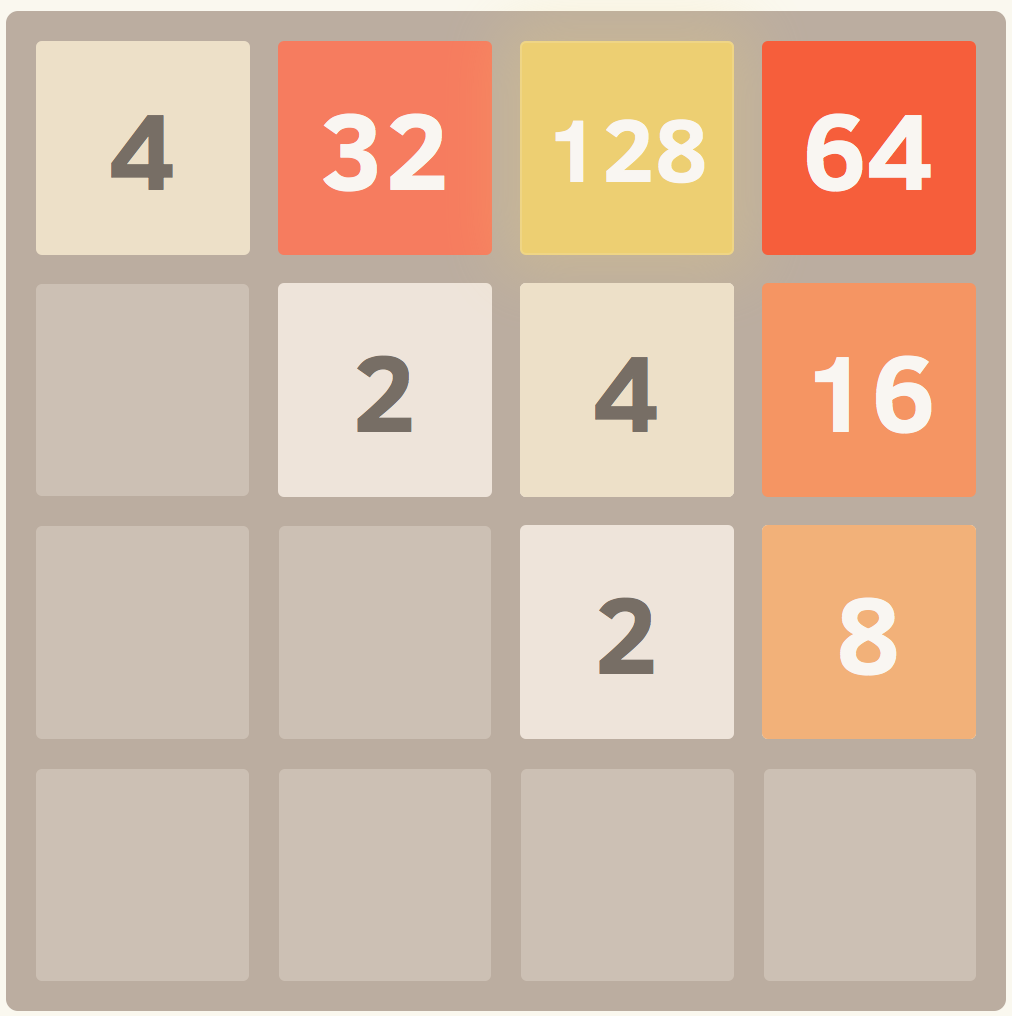
\includegraphics[scale=0.35]{img/2048board}
\caption{The board of 2048, after a couple of moves}
\label{fig:2048}
\end{figure}

\section{Background Information}
This section explains the basics of the techniques we will be using in our algorithm, to help our agent learn how to play the game 2048.
 
\subsection{Reinforcement Learning}
When an agent interacts with an environment, and it receives a reward for this action, he will be able to distinguish between good, and bad actions based on this reward. This is what we call reinforcement learning \cite{sutton1998rl}, which we can define as a Markov decision process \cite{howard1960mdp}, that is a 5-tuple $(S, A, P, R, \gamma)$ where:
\begin{itemize}
\item $S$ is a finite set that contains the states of the environment
\item $A$ is a continuous set with actions available in each state
\item $P$ is the probability distribution that assigns a probability to each state, action pair $(S$ x $A) \mapsto [0,1]$
\item $R$ contains the expected immediate rewards (given) for performing an action in a state $(S$ x $A) \mapsto \mathbb{R}$
\item $\gamma$ is the discount factor
\end{itemize}
From the environment an agent will perceive the state $s_{i} \in S$ he is in. Bounded to this state a set of actions $A_{i} \subset A$ that the agent can choose to perform. The agent has a policy $\pi$ that decides which action the agent is going to take. For each state-action pair $(s_{i}, a_{j})$ the agent will receive a reward $r$, and uses this reward to update its policy, such that it will learn how to maximize the cumulative sum of rewards. Thus if we would perform an action $a_{j}$, in a state $s_{i}$, and would be returned a positive reward $r$ the probability of choosing that action $a_{j}$ would increase. The agent does not need to know beforehand which actions are good, and which actions are bad, he learns this by interacting with the environment, and it is in there that the power of RL lies.

\subsubsection{Q-Learning}
One of the best-known algorithms to solve a RL problem is the Q-learning algorithm \cite{sutton1998rl}.
\begin{equation}
Q(s_{t}, a_{t}) \gets Q(s_{t}, a_{t}) + \alpha[r_{t+1} + \gamma\smash{\displaystyle\max_{a}} Q(s_{t+1}, a) - Q(s_{t}, a_{t})]
\label{eq:qlearning}
\end{equation}
Using this algorithm, we learn an action-value function, from which we receive the expected utility for each state-action pair. After having learned this function, the optimal policy will then be selecting the action with the highest $Q-value$ in each state. Equation~\ref{eq:qlearning} shows us how we update these $Q-values$, which has 3 influential parameters.\\
\textbf{Reward} $r$ is the value our MDP returns when we perform an action in a state. The higher this reward is for our chosen action, the better that action was compared to the others.\\
\textbf{Discount factor} $\gamma$ has an influence on how important the future rewards are for our function. For a value of 0 only the current returned reward would be important, while for a high value (close to 1) we would look for a high reward in the long run.\\
\textbf{Learning rate} $\alpha$ has an influence on how much we $learn$ by performing an action. If $\alpha=0$ we would not learn anything, while for $\alpha=1$ the new information would practically overwrite the old one. We have to find a tradeoff between learning nothing, and only remember the last information received.

\subsubsection{Generalization and Function Approximation}
Previously we made the assumption that it was possible to save the $Q-values$ for each state-action pair, but this is not possible when our state-, or action space becomes large or continuous. Therefore we try to generalize states that are similar, and use function approximation to find the optimal policy. 

\subsubsection{Tile Coding}
A well-known technique is Tile Coding \cite{sutton1998rl}, where use multiple grids of tiles as a layer over our state space. Each grid, also called $tiling$, represents a feature vector, and each tile thus symbolizes a binary feature. The bigger a tile is, the more we generalize. We give weights to each tiling, and can simply use the weighted sum approach to calculate the approximate value function. This set of weights has to be tuned to find the best approximation. Figure~\ref{fig:figtmp54} shows a graphical representation of such a grid tiles over a state space.
\begin{figure}[H]
\centering
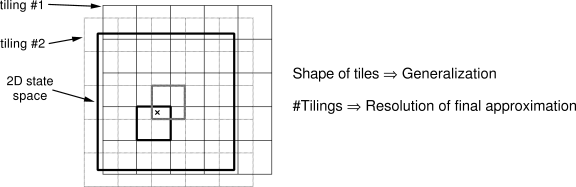
\includegraphics[width=\textwidth]{img/figtmp54}
\caption{Representation of grid tilings, taken from \cite{sutton1998rl}}
\label{fig:figtmp54}
\end{figure}

\subsection{Artificial Neural Networks}
A well known family of modeling techniques is are the Artificial Neural Networks (ANN). They are inspired by biological neural networks as can be found within the human brain. An ANN consists of distributed, interconnected nodes, called `neurons'. Each neuron performs parallel a logistic function with the input it receives (from other neurons or input data) and produces the output of this function which will be sent to other neurons within the network or serves as the output of the network. Many different architectures exist. 

\subsubsection{Using ANN for RL}
In most cases ANN is used for supervised learning, where we are given a dataset consisting of an input $x$, and an outcome $y$, where we try to learn the function $f:X \mapsto Y$. This is different for RL problems, here we perform an action $a$, within a state $s$, and are returned a reward $r$. We can translate this to the supervised learning example, our state-action pair $(s,a)$ is our input $x$, and the returned reward $r$, is our outcome $y$. Since our problem consists of a continuous space, and we have to use function approximation to find the optimal policy, it is clear that we can use ANN for this. It has been shown that ANN can be used with RL \cite{dominic1991ann,hoskins1992ann} multiple times, and more recently also on problems with a continuous space \cite{wang2005ann}.
\section{Methods}
In detail de methodes bespreken die we gebruiken, de functionaliteiten, eigenschappen en zo

\section{Experimental setup}
Het probleem 2048 goed uitleggen, en als we parameters in onze functies hebben, zeggen waarom die gekozen en zo.

\section{Results}
Resultaten tonen, en bespreken
\section{Discussion and Future work}
Praten over het nut van dit, wat het opgeleverd heeft, en hoe we het kunnen verbeteren in de toekomst
\section{Acknowledgement}
This paper was realized for the Current Trends in Artificial Intelligence course between the VUB, and ULB.
We would like to thank Professor Hugues Bersini, and Assistant Johan Loeckx for the interesting presentations they arranged for this course, and all the information it taught us.
\nocite{*}
\bibliographystyle{plain}
\bibliography{article}
\end{document}